\documentclass[oneside]{book}

% Packages required by doxygen
\usepackage{calc}
\usepackage{doxygen}
\usepackage{graphicx}
\usepackage[utf8]{inputenc}
\usepackage{makeidx}
\usepackage{multicol}
\usepackage{multirow}
\usepackage{textcomp}
\usepackage[table]{xcolor}

% NLS support packages
\usepackage{polski}
\usepackage[T1]{fontenc}

% Font selection
\usepackage[T1]{fontenc}
\usepackage{mathptmx}
\usepackage[scaled=.90]{helvet}
\usepackage{courier}
\usepackage{amssymb}
\usepackage{sectsty}
\renewcommand{\familydefault}{\sfdefault}
\allsectionsfont{%
  \fontseries{bc}\selectfont%
  \color{darkgray}%
}
\renewcommand{\DoxyLabelFont}{%
  \fontseries{bc}\selectfont%
  \color{darkgray}%
}

% Page & text layout
\usepackage{geometry}
\geometry{%
  a4paper,%
  top=2.5cm,%
  bottom=2.5cm,%
  left=2.5cm,%
  right=2.5cm%
}
\tolerance=750
\hfuzz=15pt
\hbadness=750
\setlength{\emergencystretch}{15pt}
\setlength{\parindent}{0cm}
\setlength{\parskip}{0.2cm}
\makeatletter
\renewcommand{\paragraph}{%
  \@startsection{paragraph}{4}{0ex}{-1.0ex}{1.0ex}{%
    \normalfont\normalsize\bfseries\SS@parafont%
  }%
}
\renewcommand{\subparagraph}{%
  \@startsection{subparagraph}{5}{0ex}{-1.0ex}{1.0ex}{%
    \normalfont\normalsize\bfseries\SS@subparafont%
  }%
}
\makeatother

% Headers & footers
\usepackage{fancyhdr}
\pagestyle{fancyplain}
\fancyhead[LE]{\fancyplain{}{\bfseries\thepage}}
\fancyhead[CE]{\fancyplain{}{}}
\fancyhead[RE]{\fancyplain{}{\bfseries\leftmark}}
\fancyhead[LO]{\fancyplain{}{\bfseries\rightmark}}
\fancyhead[CO]{\fancyplain{}{}}
\fancyhead[RO]{\fancyplain{}{\bfseries\thepage}}
\fancyfoot[LE]{\fancyplain{}{}}
\fancyfoot[CE]{\fancyplain{}{}}
\fancyfoot[RE]{\fancyplain{}{\bfseries\scriptsize Wygenerowano Cz, 19 sty 2017 07\-:29\-:20 dla Menu programem Doxygen }}
\fancyfoot[LO]{\fancyplain{}{\bfseries\scriptsize Wygenerowano Cz, 19 sty 2017 07\-:29\-:20 dla Menu programem Doxygen }}
\fancyfoot[CO]{\fancyplain{}{}}
\fancyfoot[RO]{\fancyplain{}{}}
\renewcommand{\footrulewidth}{0.4pt}
\renewcommand{\chaptermark}[1]{%
  \markboth{#1}{}%
}
\renewcommand{\sectionmark}[1]{%
  \markright{\thesection\ #1}%
}

% Indices & bibliography
\usepackage{natbib}
\usepackage[titles]{tocloft}
\setcounter{tocdepth}{3}
\setcounter{secnumdepth}{5}
\makeindex

% Hyperlinks (required, but should be loaded last)
\usepackage{ifpdf}
\ifpdf
  \usepackage[pdftex,pagebackref=true]{hyperref}
\else
  \usepackage[ps2pdf,pagebackref=true]{hyperref}
\fi
\hypersetup{%
  colorlinks=true,%
  linkcolor=blue,%
  citecolor=blue,%
  unicode%
}

% Custom commands
\newcommand{\clearemptydoublepage}{%
  \newpage{\pagestyle{empty}\cleardoublepage}%
}


%===== C O N T E N T S =====

\begin{document}

% Titlepage & ToC
\hypersetup{pageanchor=false}
\pagenumbering{roman}
\begin{titlepage}
\vspace*{7cm}
\begin{center}%
{\Large Menu }\\
\vspace*{1cm}
{\small Marta Pacuszka}\\
\end{center}
\end{titlepage}
\clearemptydoublepage
\tableofcontents
\clearemptydoublepage
\pagenumbering{arabic}
\hypersetup{pageanchor=true}

%--- Begin generated contents ---
\chapter{Informacje o projekcie}
\label{md_README}
\hypertarget{md_README}{}
\section*{Polecenie}

Menu programu okienkowego jest kolekcją wyborów. Każdy z wyborów jest albo jednoznaczny albo wskazuje na inne menu. Oprogramować bibliotekę klas reprezentujących menu. Biblioteka ma umożliwiać następujące czynności\-:
\begin{DoxyItemize}
\item Dodawanie/usuwanie wyborów jednoznacznych do/z (pod)menu.
\item Dodawanie/usuwanie podmenu do/z (pod)menu.
\item Przypisywanie wyborów jednoznacznych do pewnych funkcji.
\item Rozwijanie/zwijanie podmenu.
\item Dokonywanie wyborów jednoznacznych. Napisać program, który wszystkie powyższe funkcjonalności udostępnia poprzez polecenia wydawane z klawiatury. Przyjąć, że za wyborami jednoznacznymi może kryć się stały zbiór funkcji wypisujący na konsoli komunikaty typu “\-Zadziałała funkcja nr 14”.
\end{DoxyItemize}

\section*{Założenia}


\begin{DoxyEnumerate}
\item Menu zawsze musi się składać z conajmniej jednego Wyboru typu \hyperlink{classPodmenu}{Podmenu}. Nie można usunąć takiego \hyperlink{classPodmenu}{Podmenu}.
\item Usunięcie \hyperlink{classPodmenu}{Podmenu} oznacza usunięcie razem z nim wszystkich zagnieżdżonych w nim Wyborów.
\item Po usunięciu elementu (elementów) Menu kursor wskazuje na następny obiekt.
\item Jeżeli \hyperlink{classPodmenu}{Podmenu} jest zwinięte, nie ma możliwości przejścia kursorem do któregokolwiek z zagnieżdżonych w nim Wyborów. W tym celu należy je najpierw rozwinąć.
\end{DoxyEnumerate}

\section*{Struktura klas reprezentujących Menu}

Lista klas w kolejności nadrzędności, tzn. klasa wymieniona jako pierwsza nie korzysta z żadnej z innych klas, jest za to wykorzystywana przez klasy nadrzędne, w szczególności przez klasę bezpośrednio nadrzędną, tzn. klasę o numerze 2.


\begin{DoxyEnumerate}
\item \hyperlink{classWybor}{Wybor}
\begin{DoxyItemize}
\item \hyperlink{classJednoznaczny}{Jednoznaczny}
\item \hyperlink{classPodmenu}{Podmenu}
\end{DoxyItemize}
\item \hyperlink{classKolekcja}{Kolekcja}
\item \hyperlink{classObsluga}{Obsluga}
\item \hyperlink{classInterfejs}{Interfejs} 
\end{DoxyEnumerate}
\chapter{Dokumentacja klas}
\hypertarget{classWybor}{\section{Dokumentacja klasy Wybor}
\label{classWybor}\index{Wybor@{Wybor}}
}


{\ttfamily \#include $<$wybor.\-h$>$}

Diagram dziedziczenia dla Wybor\begin{figure}[H]
\begin{center}
\leavevmode
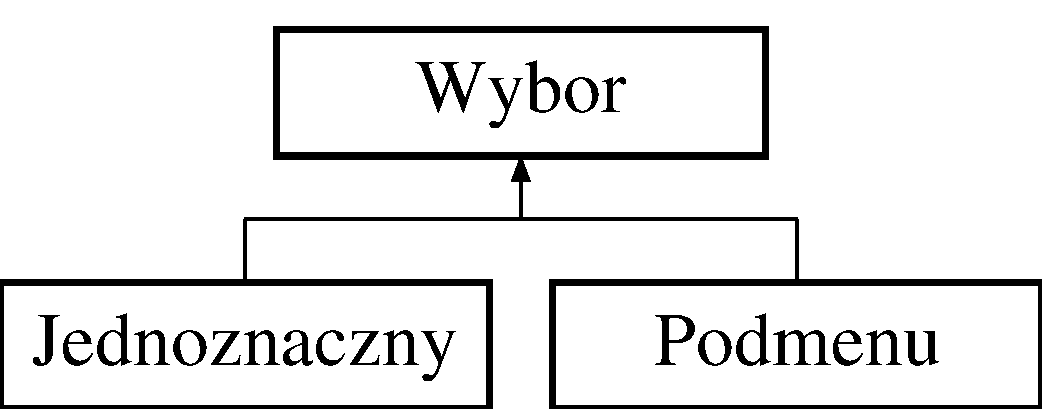
\includegraphics[height=2.000000cm]{classWybor}
\end{center}
\end{figure}
\subsection*{Metody publiczne}
\begin{DoxyCompactItemize}
\item 
\hypertarget{classWybor_a3e0c715881bdeeec7bbcb84531e3b0e5}{{\bfseries Wybor} (std\-::string s)}\label{classWybor_a3e0c715881bdeeec7bbcb84531e3b0e5}

\end{DoxyCompactItemize}
\subsection*{Metody chronione}
\begin{DoxyCompactItemize}
\item 
\hypertarget{classWybor_a78db78719c9fc86ad4c3a213397baf54}{int {\bfseries Jaki\-Stopien\-Zagniezdzenia} ()}\label{classWybor_a78db78719c9fc86ad4c3a213397baf54}

\item 
\hypertarget{classWybor_a67fe9d804ece1158b6b45d42875b05af}{void {\bfseries Ukryj} ()}\label{classWybor_a67fe9d804ece1158b6b45d42875b05af}

\item 
\hypertarget{classWybor_a22198d1190c37209a2db625a3e3b0fef}{void {\bfseries Pokaz} ()}\label{classWybor_a22198d1190c37209a2db625a3e3b0fef}

\item 
\hypertarget{classWybor_a76709c72cad50840901fcdb8ee365f1f}{bool {\bfseries hidden} ()}\label{classWybor_a76709c72cad50840901fcdb8ee365f1f}

\item 
\hypertarget{classWybor_a3257df3c35728ec264a51dce3ac28f55}{void {\bfseries Nadaj\-Stopien\-Zagniezdzenia} (int n)}\label{classWybor_a3257df3c35728ec264a51dce3ac28f55}

\item 
\hypertarget{classWybor_a42cb8cae1bafe052a3b96eddee87de62}{virtual void {\bfseries Wypisz} (std\-::ostream \&ekran)}\label{classWybor_a42cb8cae1bafe052a3b96eddee87de62}

\end{DoxyCompactItemize}
\subsection*{Atrybuty chronione}
\begin{DoxyCompactItemize}
\item 
\hypertarget{classWybor_ada1632e8ce78ba40ea8f491f2db66b77}{std\-::string {\bfseries nazwa}}\label{classWybor_ada1632e8ce78ba40ea8f491f2db66b77}

\item 
\hypertarget{classWybor_aee3503d5cc003f8dd73547fe4e58cef9}{int {\bfseries stopien\-Zagniezdzenia}}\label{classWybor_aee3503d5cc003f8dd73547fe4e58cef9}

\item 
\hypertarget{classWybor_a946727299ecc881dc13ac30e1d9f33d8}{bool {\bfseries czy\-Ukryty}}\label{classWybor_a946727299ecc881dc13ac30e1d9f33d8}

\end{DoxyCompactItemize}
\subsection*{Przyjaciele}
\begin{DoxyCompactItemize}
\item 
\hypertarget{classWybor_acbfbc86fbec88d567dc6313b7419d6fa}{class {\bfseries Kolekcja}}\label{classWybor_acbfbc86fbec88d567dc6313b7419d6fa}

\item 
\hypertarget{classWybor_aaba4100c363553c323b55344e224e15d}{class {\bfseries Obsluga}}\label{classWybor_aaba4100c363553c323b55344e224e15d}

\item 
\hypertarget{classWybor_a1181e1d648ce67ab4f131a6f1639c6fd}{std\-::ostream \& {\bfseries operator$<$$<$} (std\-::ostream \&ekran, \hyperlink{classWybor}{Wybor} \&w)}\label{classWybor_a1181e1d648ce67ab4f131a6f1639c6fd}

\end{DoxyCompactItemize}


\subsection{Opis szczegółowy}
Klasa reprezentująca pojedynczy wybór -\/ jest klasą bazową dla klas reprezentujących wybory jednoznaczne i podmenu . Z jej obiektów korzysta zaprzyjaźniona klasa \hyperlink{classKolekcja}{Kolekcja}. Klasa przechowuje takie informacje o wyborze, jak jego nazwa czy stopień zagnieżdżenia. 
\hypertarget{classPodmenu}{\section{Dokumentacja klasy Podmenu}
\label{classPodmenu}\index{Podmenu@{Podmenu}}
}


{\ttfamily \#include $<$wybor.\-h$>$}

Diagram dziedziczenia dla Podmenu\begin{figure}[H]
\begin{center}
\leavevmode
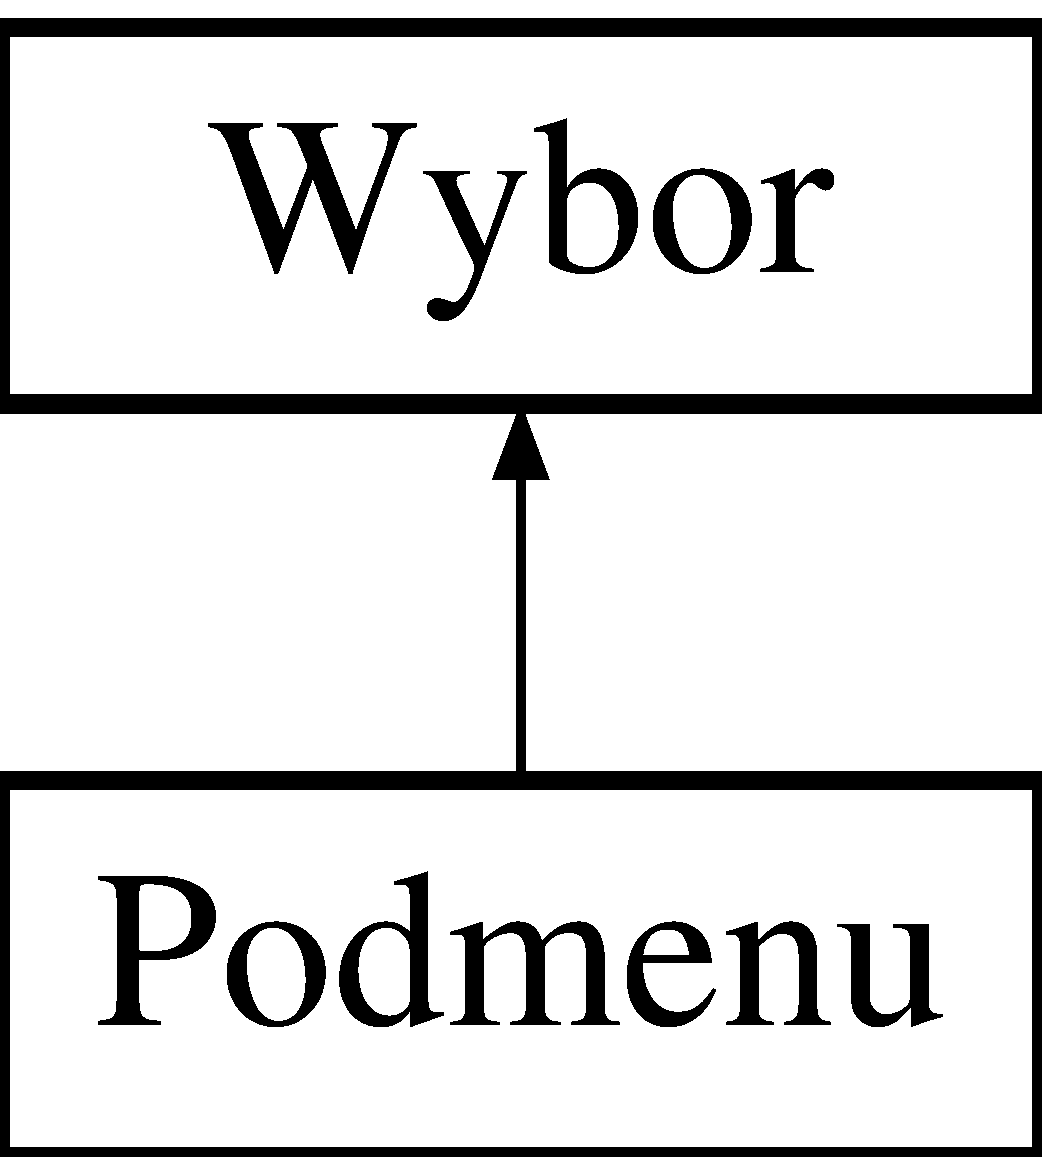
\includegraphics[height=2.000000cm]{classPodmenu}
\end{center}
\end{figure}
\subsection*{Metody publiczne}
\begin{DoxyCompactItemize}
\item 
\hypertarget{classPodmenu_a959a79e13f3498087b22952da8b38baa}{{\bfseries Podmenu} (std\-::string s)}\label{classPodmenu_a959a79e13f3498087b22952da8b38baa}

\end{DoxyCompactItemize}
\subsection*{Przyjaciele}
\begin{DoxyCompactItemize}
\item 
\hypertarget{classPodmenu_acbfbc86fbec88d567dc6313b7419d6fa}{class {\bfseries Kolekcja}}\label{classPodmenu_acbfbc86fbec88d567dc6313b7419d6fa}

\item 
\hypertarget{classPodmenu_aaba4100c363553c323b55344e224e15d}{class {\bfseries Obsluga}}\label{classPodmenu_aaba4100c363553c323b55344e224e15d}

\end{DoxyCompactItemize}
\subsection*{Dodatkowe Dziedziczone Składowe}


\subsection{Opis szczegółowy}
Klasa dziedzicząca z klasy Wybór. Obiekty tej klasy reprezentują \hyperlink{classPodmenu}{Podmenu} -\/ Wybór, w którym można zagnieżdżać inne Wybory (o wyższym stopniu zagnieżdżenia). 
\hypertarget{classJednoznaczny}{\section{Dokumentacja klasy Jednoznaczny}
\label{classJednoznaczny}\index{Jednoznaczny@{Jednoznaczny}}
}


{\ttfamily \#include $<$wybor.\-h$>$}

Diagram dziedziczenia dla Jednoznaczny\begin{figure}[H]
\begin{center}
\leavevmode
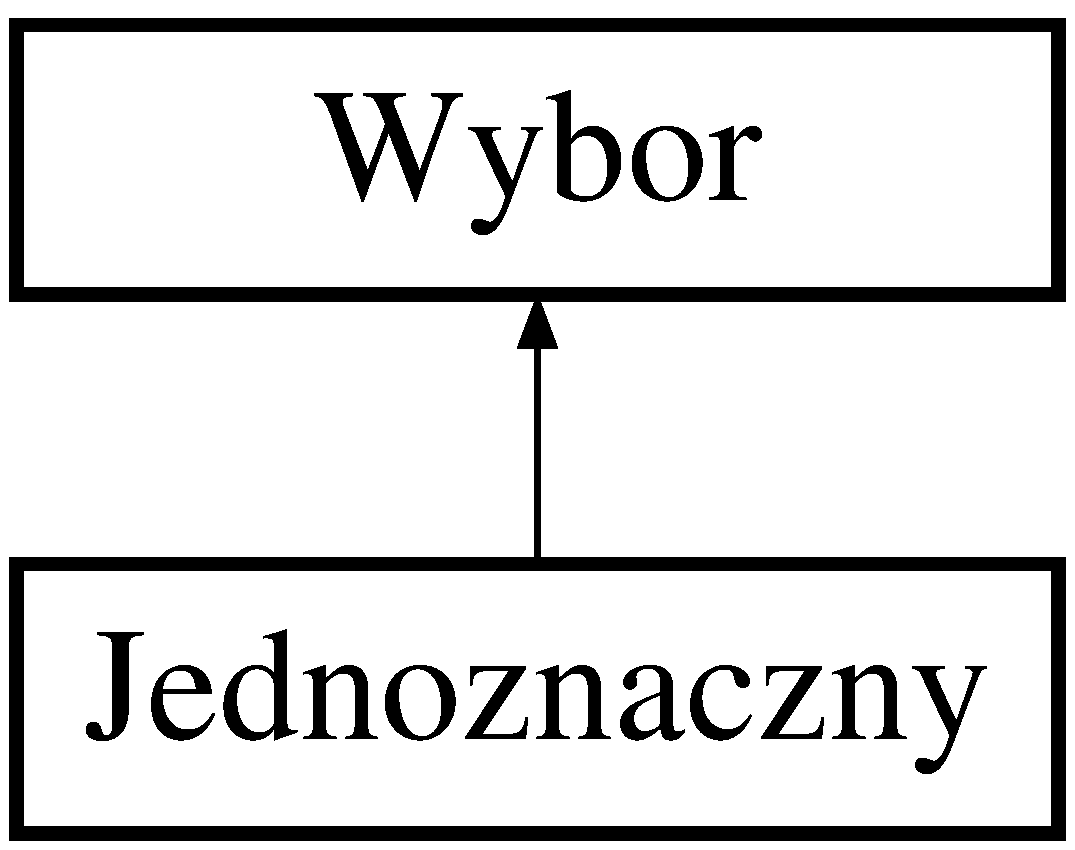
\includegraphics[height=2.000000cm]{classJednoznaczny}
\end{center}
\end{figure}
\subsection*{Metody publiczne}
\begin{DoxyCompactItemize}
\item 
\hypertarget{classJednoznaczny_a132863c0ea5e199f3e03b77eaae29b6f}{{\bfseries Jednoznaczny} (std\-::string s)}\label{classJednoznaczny_a132863c0ea5e199f3e03b77eaae29b6f}

\end{DoxyCompactItemize}
\subsection*{Przyjaciele}
\begin{DoxyCompactItemize}
\item 
\hypertarget{classJednoznaczny_acbfbc86fbec88d567dc6313b7419d6fa}{class {\bfseries Kolekcja}}\label{classJednoznaczny_acbfbc86fbec88d567dc6313b7419d6fa}

\item 
\hypertarget{classJednoznaczny_aaba4100c363553c323b55344e224e15d}{class {\bfseries Obsluga}}\label{classJednoznaczny_aaba4100c363553c323b55344e224e15d}

\end{DoxyCompactItemize}
\subsection*{Dodatkowe Dziedziczone Składowe}


\subsection{Opis szczegółowy}
Klasa dziedzicząca z klasy Wybór. Obiekty tej klasy reprezentują Wybór \hyperlink{classJednoznaczny}{Jednoznaczny}. Poza polami i metodami dziedziczonymi, posiada swoje własne, charakterystyczne dla siebie metody i pola związane z przypisywaniem do wyborów jednoznacznych konkretnych funkcji. 
\hypertarget{classKolekcja}{\section{Dokumentacja klasy Kolekcja}
\label{classKolekcja}\index{Kolekcja@{Kolekcja}}
}


{\ttfamily \#include $<$kolekcja.\-h$>$}

\subsection*{Metody publiczne}
\begin{DoxyCompactItemize}
\item 
\hypertarget{classKolekcja_a69ee9233ae5b67dadc29bd8c038e017d}{{\bfseries Kolekcja} (std\-::string s)}\label{classKolekcja_a69ee9233ae5b67dadc29bd8c038e017d}

\end{DoxyCompactItemize}
\subsection*{Przyjaciele}
\begin{DoxyCompactItemize}
\item 
\hypertarget{classKolekcja_aaba4100c363553c323b55344e224e15d}{class {\bfseries Obsluga}}\label{classKolekcja_aaba4100c363553c323b55344e224e15d}

\end{DoxyCompactItemize}


\subsection{Opis szczegółowy}
Klasa zaprzyjaźniona z klasą Wybór i klasami pochodnymi, obsługująca obiekty tej klasy. Wybory są przechowywane w liście Zbior\-Wyborow.

Zgodnie z założeniem, że każda \hyperlink{classKolekcja}{Kolekcja} musi posiadać jeden obiekt klasy \hyperlink{classPodmenu}{Podmenu}, jej konstruktor tworzy nowy obiekt klasy \hyperlink{classPodmenu}{Podmenu} o stopniu zagnieżdżenia 0 i dodaje go na początek listy Zbiór\-Wyborow. Nazwa tego obiektu klasy \hyperlink{classPodmenu}{Podmenu} jest jednocześnie nazwą całej kolekcji. 
\hypertarget{classObsluga}{\section{Dokumentacja klasy Obsluga}
\label{classObsluga}\index{Obsluga@{Obsluga}}
}


{\ttfamily \#include $<$obsluga.\-h$>$}

\subsection*{Metody publiczne}
\begin{DoxyCompactItemize}
\item 
\hypertarget{classObsluga_a5d6c171d6a9b4f6f9caa444b09fcb460}{{\bfseries Obsluga} (std\-::string s)}\label{classObsluga_a5d6c171d6a9b4f6f9caa444b09fcb460}

\item 
void \hyperlink{classObsluga_aaf91f84ea408e2ee478009ff28d0719c}{Dodaj\-Menu} (std\-::string s)
\item 
void \hyperlink{classObsluga_a141f1c29476498fecf4c74983c60f107}{Dodaj\-Wybor\-Jedn} (std\-::string s)
\item 
void \hyperlink{classObsluga_a79ac7b11058423a625c971688d012a5c}{Przypisz\-Funkcje} (int n)
\item 
void \hyperlink{classObsluga_af4498067cfb12688c9b395a9ec58cd4a}{Usun} ()
\item 
void \hyperlink{classObsluga_a5567d2685b8ca89fe1d6593f0826a653}{Dalej} ()
\item 
void \hyperlink{classObsluga_a36f1c6f4841b40c6d44fd1fc3fd2449b}{Wstecz} ()
\item 
void \hyperlink{classObsluga_add7a400f68afe5e0c049855ed428fd3a}{Zwin} ()
\item 
void \hyperlink{classObsluga_a3b625d79bab85d07a4da24bc105e312d}{Rozwin} ()
\item 
void \hyperlink{classObsluga_aed45a6c9be358bcbce191617e6e04be7}{Wykonaj} ()
\end{DoxyCompactItemize}
\subsection*{Przyjaciele}
\begin{DoxyCompactItemize}
\item 
\hypertarget{classObsluga_a29bee9078fbc123e023d6d8cb376928d}{class {\bfseries Interfejs}}\label{classObsluga_a29bee9078fbc123e023d6d8cb376928d}

\item 
\hypertarget{classObsluga_aeac69cdc1820ab17cd012468f3f0a85c}{std\-::ostream \& {\bfseries operator$<$$<$} (std\-::ostream \&ekran, \hyperlink{classObsluga}{Obsluga} \&m)}\label{classObsluga_aeac69cdc1820ab17cd012468f3f0a85c}

\end{DoxyCompactItemize}


\subsection{Opis szczegółowy}
Klasa obsługująca obiekt klasy \hyperlink{classKolekcja}{Kolekcja}. Potrafi modyfikować obiekty klasy Wybór, przechowywane przez atrybut klasy \hyperlink{classKolekcja}{Kolekcja}. Umożliwia wykonywanie operacji na Kolekcji -\/ dodawanie Wyborów, zwijanie i rozwijanie \hyperlink{classPodmenu}{Podmenu} oraz swobodne poruszanie się po kolejnych Wyborach, z uwzględnieniem omijania Wyborów ukrytych. 

\subsection{Dokumentacja funkcji składowych}
\hypertarget{classObsluga_a5567d2685b8ca89fe1d6593f0826a653}{\index{Obsluga@{Obsluga}!Dalej@{Dalej}}
\index{Dalej@{Dalej}!Obsluga@{Obsluga}}
\subsubsection[{Dalej}]{\setlength{\rightskip}{0pt plus 5cm}void Obsluga\-::\-Dalej (
\begin{DoxyParamCaption}
{}
\end{DoxyParamCaption}
)}}\label{classObsluga_a5567d2685b8ca89fe1d6593f0826a653}
Przesuwa kursor na kolejny element listy Zbior\-Wyborow. Uwzględnia fakt, że część elementów może być ukryta i pomija je. Gdy Kursor pokazuje na ostatni element, przesuwa go na początek. \hypertarget{classObsluga_aaf91f84ea408e2ee478009ff28d0719c}{\index{Obsluga@{Obsluga}!Dodaj\-Menu@{Dodaj\-Menu}}
\index{Dodaj\-Menu@{Dodaj\-Menu}!Obsluga@{Obsluga}}
\subsubsection[{Dodaj\-Menu}]{\setlength{\rightskip}{0pt plus 5cm}void Obsluga\-::\-Dodaj\-Menu (
\begin{DoxyParamCaption}
\item[{std\-::string}]{s}
\end{DoxyParamCaption}
)}}\label{classObsluga_aaf91f84ea408e2ee478009ff28d0719c}
Metoda tworząca nowy obiekt typu \hyperlink{classPodmenu}{Podmenu} i dodająca go do listy Zbior\-Wyborow zaraz za elementej tej listy pokazywanym przez atrybut Kursor. 
\begin{DoxyParams}{Parametry}
{\em s} & nazwa obiektu typu \hyperlink{classPodmenu}{Podmenu}\\
\hline
\end{DoxyParams}
\hypertarget{classObsluga_a141f1c29476498fecf4c74983c60f107}{\index{Obsluga@{Obsluga}!Dodaj\-Wybor\-Jedn@{Dodaj\-Wybor\-Jedn}}
\index{Dodaj\-Wybor\-Jedn@{Dodaj\-Wybor\-Jedn}!Obsluga@{Obsluga}}
\subsubsection[{Dodaj\-Wybor\-Jedn}]{\setlength{\rightskip}{0pt plus 5cm}void Obsluga\-::\-Dodaj\-Wybor\-Jedn (
\begin{DoxyParamCaption}
\item[{std\-::string}]{s}
\end{DoxyParamCaption}
)}}\label{classObsluga_a141f1c29476498fecf4c74983c60f107}
Metoda tworząca nowy obiekt typu \hyperlink{classJednoznaczny}{Jednoznaczny} i dodająca go do listy Zbior\-Wyborow zaraz za elementej tej listy pokazywanym przez atrybut Kursor. 
\begin{DoxyParams}{Parametry}
{\em s} & nazwa obiektu typu \hyperlink{classJednoznaczny}{Jednoznaczny}\\
\hline
\end{DoxyParams}
\hypertarget{classObsluga_a79ac7b11058423a625c971688d012a5c}{\index{Obsluga@{Obsluga}!Przypisz\-Funkcje@{Przypisz\-Funkcje}}
\index{Przypisz\-Funkcje@{Przypisz\-Funkcje}!Obsluga@{Obsluga}}
\subsubsection[{Przypisz\-Funkcje}]{\setlength{\rightskip}{0pt plus 5cm}void Obsluga\-::\-Przypisz\-Funkcje (
\begin{DoxyParamCaption}
\item[{int}]{n}
\end{DoxyParamCaption}
)}}\label{classObsluga_a79ac7b11058423a625c971688d012a5c}
Przypisuje do odpowiedniego pola obiektu typu \hyperlink{classJednoznaczny}{Jednoznaczny} wskaźnik na funkcję, którą ma wywoływać ten Wybór. 
\begin{DoxyParams}{Parametry}
{\em n} & numer funkcji, która ma zostać przypisana Wyborowi\\
\hline
\end{DoxyParams}
\hypertarget{classObsluga_a3b625d79bab85d07a4da24bc105e312d}{\index{Obsluga@{Obsluga}!Rozwin@{Rozwin}}
\index{Rozwin@{Rozwin}!Obsluga@{Obsluga}}
\subsubsection[{Rozwin}]{\setlength{\rightskip}{0pt plus 5cm}void Obsluga\-::\-Rozwin (
\begin{DoxyParamCaption}
{}
\end{DoxyParamCaption}
)}}\label{classObsluga_a3b625d79bab85d07a4da24bc105e312d}
Metoda pokazuje wszystkie elementy Kolekcji zagnieżdżone w \hyperlink{classPodmenu}{Podmenu} (jeżeli były wcześniej ukryte). Jeżeli \hyperlink{classPodmenu}{Podmenu} nie jest zwinięte, zgłasza wyjątek. Jeżeli wywołane dla typu innego niż \hyperlink{classPodmenu}{Podmenu}, zgłasza wyjątek. \hypertarget{classObsluga_af4498067cfb12688c9b395a9ec58cd4a}{\index{Obsluga@{Obsluga}!Usun@{Usun}}
\index{Usun@{Usun}!Obsluga@{Obsluga}}
\subsubsection[{Usun}]{\setlength{\rightskip}{0pt plus 5cm}void Obsluga\-::\-Usun (
\begin{DoxyParamCaption}
{}
\end{DoxyParamCaption}
)}}\label{classObsluga_af4498067cfb12688c9b395a9ec58cd4a}
Usuwa Wybór, na który aktualnie wskazuje Kursor wraz ze wszystkimi Wyborami zagnieżdżonymi. Kursor na koniec jest ustawiony na poprzednim obiekcie. \hypertarget{classObsluga_a36f1c6f4841b40c6d44fd1fc3fd2449b}{\index{Obsluga@{Obsluga}!Wstecz@{Wstecz}}
\index{Wstecz@{Wstecz}!Obsluga@{Obsluga}}
\subsubsection[{Wstecz}]{\setlength{\rightskip}{0pt plus 5cm}void Obsluga\-::\-Wstecz (
\begin{DoxyParamCaption}
{}
\end{DoxyParamCaption}
)}}\label{classObsluga_a36f1c6f4841b40c6d44fd1fc3fd2449b}
Przesuwa kursor na poprzedni element listy Zbior\-Wyborow. Uwzględnia fakt, że część elementów może być ukryta i pomija je. Gdy Kursor pokazuje na pierwszy element, przesuwa go na koniec. \hypertarget{classObsluga_aed45a6c9be358bcbce191617e6e04be7}{\index{Obsluga@{Obsluga}!Wykonaj@{Wykonaj}}
\index{Wykonaj@{Wykonaj}!Obsluga@{Obsluga}}
\subsubsection[{Wykonaj}]{\setlength{\rightskip}{0pt plus 5cm}void Obsluga\-::\-Wykonaj (
\begin{DoxyParamCaption}
{}
\end{DoxyParamCaption}
)}}\label{classObsluga_aed45a6c9be358bcbce191617e6e04be7}
Metoda wywoływana dla obiektu klasy \hyperlink{classJednoznaczny}{Jednoznaczny} (dla każdego innego zgłasza wyjątek). Wywołuje funkcję przypisaną do Wyboru Jednoznacznego pokazywanego przez Kursor. Jeżeli funkcja nie została jeszcze przypisana, zgłasza wyjątek. \hypertarget{classObsluga_add7a400f68afe5e0c049855ed428fd3a}{\index{Obsluga@{Obsluga}!Zwin@{Zwin}}
\index{Zwin@{Zwin}!Obsluga@{Obsluga}}
\subsubsection[{Zwin}]{\setlength{\rightskip}{0pt plus 5cm}void Obsluga\-::\-Zwin (
\begin{DoxyParamCaption}
{}
\end{DoxyParamCaption}
)}}\label{classObsluga_add7a400f68afe5e0c049855ed428fd3a}
Metoda ukrywa wszystkie elementy Kolekcji zagnieżdżone w \hyperlink{classPodmenu}{Podmenu}. Jeżeli wywołane dla typu innego niż \hyperlink{classPodmenu}{Podmenu}, zgłasza wyjątek. 
\hypertarget{classInterfejs}{\section{Dokumentacja klasy Interfejs}
\label{classInterfejs}\index{Interfejs@{Interfejs}}
}


{\ttfamily \#include $<$interfejs.\-h$>$}

\subsection*{Metody publiczne}
\begin{DoxyCompactItemize}
\item 
void \hyperlink{classInterfejs_ab016a2fdc6ba2553378167d6a07f8ea3}{Start} ()
\item 
void \hyperlink{classInterfejs_a46d175ac6f4e02e5e60fea8bb54c98b7}{Program} (\hyperlink{classObsluga}{Obsluga} \&M)
\end{DoxyCompactItemize}


\subsection{Opis szczegółowy}
Klasa reprezentująca interfejs użytkownika. Menu wyświetlane jest w terminalu w następujący umówny sposób\-:
\begin{DoxyItemize}
\item Poziom zagnieżdżenia reprezentowany jest odpowiednim wcięciem.
\item Pozycja Kursora pokazywana jest symbolem $\ast$$\ast$$\ast$.
\item Lista dostępnych poleceń wyświetlana jest bezpośrednio pod Menu.
\item \hyperlink{classPodmenu}{Podmenu} reprezentowane jest zapisem\-: {\bfseries $\vert$ Nazwa podmenu }, gdy menu nie posiada zagnieżdżonych obiektów lub {\bfseries $\vert$ Nazwa podmenu $\vert$}, gdy posiada zagnieżdżone obiekty (w szczególności można je rozwinąć).
\item Wybór jednoznaczny reprezentowany jest zapisem\-: {\bfseries -\/$>$ Nazwa wyboru}. Jeżeli do wyboru nie została jeszcze przypisana żadna funkcja, po dwukropku znajduje się dopisek {\bfseries funkcja nieaktywna}. 
\end{DoxyItemize}

\subsection{Dokumentacja funkcji składowych}
\hypertarget{classInterfejs_a46d175ac6f4e02e5e60fea8bb54c98b7}{\index{Interfejs@{Interfejs}!Program@{Program}}
\index{Program@{Program}!Interfejs@{Interfejs}}
\subsubsection[{Program}]{\setlength{\rightskip}{0pt plus 5cm}void Interfejs\-::\-Program (
\begin{DoxyParamCaption}
\item[{{\bf Obsluga} \&}]{M}
\end{DoxyParamCaption}
)}}\label{classInterfejs_a46d175ac6f4e02e5e60fea8bb54c98b7}
Metoda przetwarzająca polecenia uzytkownika. Może być wywołana dla stworzonego wcześniej obiektu typu \hyperlink{classObsluga}{Obsluga}. \hypertarget{classInterfejs_ab016a2fdc6ba2553378167d6a07f8ea3}{\index{Interfejs@{Interfejs}!Start@{Start}}
\index{Start@{Start}!Interfejs@{Interfejs}}
\subsubsection[{Start}]{\setlength{\rightskip}{0pt plus 5cm}void Interfejs\-::\-Start (
\begin{DoxyParamCaption}
{}
\end{DoxyParamCaption}
)}}\label{classInterfejs_ab016a2fdc6ba2553378167d6a07f8ea3}
Funkcja umożliwiająca użytkownikowi stworzenie nowego Menu od zera. Pobiera z klawiatury informacje o \hyperlink{classPodmenu}{Podmenu} o stopniu zagnieżdżenia 0, niezbędnym do utworzenia nowego obiektu typu \hyperlink{classObsluga}{Obsluga}, a następnie wywołuje funkcję \hyperlink{classInterfejs_a46d175ac6f4e02e5e60fea8bb54c98b7}{Program(\-Obsluga\& M)}. 




%--- End generated contents ---

% Index
\newpage
\phantomsection
\addcontentsline{toc}{chapter}{Indeks}
\printindex

\end{document}
